\chapter{Implementation}
In this chapter, we describe how we went about the implementation
of the debugger and reason about the design choices we made.
Also, we describe which part of the virtual machine were
modified or added for the benefit of the debugger or in
general for the greater good.

\section{T86 ISA extensions}\label{section:parser}
In chapter \todo{ref} we showed how to build a program for the T86 VM. It was
necessary to use the builder the T86 VM provides. There is currently no other
way. We remedied this with a hand-made parser of the T86 assembly language. An
example of a program for T86 is shown in figure \ref{fig:t86-program}. It is
very similar to assembly we have shown in previous sections. Thanks to this,
students can choose any language they want to implement their compiler and just
emit this assembly at the end. An unfortunate side effect is that we are no
longer able to use the \texttt{DBG} instruction. This will however be remedied
by the very debugger we are implementing here. 

Notice the \texttt{.text}, this is a section, same as the ELF format uses. We
will carry some of this over from the ELF format. Mainly, the \texttt{.text}
and \texttt{.data} sections. For debugging purposes, we will also include some
debug headers. The exact nature of this debugging headers is specified in
section \todo{ref} where the debugging information format for our debugger is
defined.

\begin{figure}
    \begin{lstlisting}
        .text

        0 MOV R0, 49
        1 PUTCHAR R0
        # Put newline
        2 MOV R0, 10
        3 PUTCHAR R0
        4 HALT
    \end{lstlisting}
    \caption{Example of an T86 program.}
    \label{fig:t86-program}
\end{figure}

We will also add a few new instructions. One is \texttt{PUTNUM}, which prints
the numerical value with a newline. This is intended as a simple debug instruction
and to ease the automated testing of the compiler. Only other way of output was
to print a char which was represented by the ascii value. If students wants
to have an automated test that his factorial program translates successfully
it is very much easier with this instruction.

Another one is the \texttt{BKPT} instruction. This instruction is similar to
\texttt{INT3} from x86\_64 or \texttt{BKPT} from ARM. It is an software
breakpoint. When the instruction is hit, a control will be passed to the
connected debugger. This is thoroughly described in the next section. 

\section{Design of the native T86 debugger}
We could simply bake the debugger into the virtual machine itself. This would
probably prove to be simplest to implement. However, the main point of the
debugger is not only to ease the code generation part, but to be a learning
point so that students might grasp how a real debugger is
implemented\footnote{The VM followed the same philosophy.}. Because of this, we
aim to simulate the real world debuggers as close as possible. The compilers
themselves may also have more targets in the future, not just the T86 VM. If we
made the debugger as part of T86 we couldn't use it for a possibly new virtual
machine. In conclusion, the virtual machine and the debugger will be two
entirely different programs, and as such, two completely different processes.

In the implementation of debugger for Linux, which was the subject of section
\todo{ref}, we described how the kernel of an operating system helps with the
implementation of the debugger via specific API. There is no operating system
between the virtual machine and the program. Still, we will strife to make the
API similar on the virtual machine part. The debugger and the VM will have to
communicate together somehow. For the interprocess comunnication, there are
several possibilities.

One of those are signals. Those however are POSIX specific. Other possibilities
are shared pipes or sockets. We choose sockets, purely because \todo{we do not
know how to use anything else :)}. Both the virtual machine and the debugger
will have an opened port through which they will communicate. The format
of the communication will be a text one, merely because of the ease of use
as opposed to binary format. The commands that the virtual machine API
will offer are
\begin{itemize}
    \item \texttt{PEEKREG x} - Return value in register \texttt{x}.
    \item \texttt{POKEREG x y} - Sets the value in register \texttt{x} to
        \texttt{y}.
    \item \texttt{PEEKDATA x} - Return value in memory at address \texttt{x}.
    \item \texttt{POKEDATA x y} - Writes a value \texttt{y} into a memory at
        address \texttt{x}.
    \item \texttt{PEEKTEXT x} - Returns instruction at address \texttt{x}.
    \item \texttt{POKETEXT x} \texttt{INS} - Rewrite the instruction at
        address
        \texttt{x} with the newly supplied instruction.
    \item \texttt{CONTINUE} - Continue the execution.
    \item \texttt{REASON} - Get the reason why the program stopped (breakpoint,
        singlestep, halt).
    \item \texttt{SINGLESTEP} - Does native level single step.
\end{itemize}
Example of how those commands can be used for communication between the virtual
machine and the debugger is shown in figure \ref{fig:dbg-vm-seq}. The interface
is similar to basic ptrace commands. We separate the memory and instruction
writing because T86 uses harvard architecture, whereas Linux doesn't separate
text and data address spaces\cite{ptrace}, so the two requests were equivalent
there.

Currently, the class that runs the program is the \texttt{Cpu}. We will add
another manager-like class. This class will take care of running the program
via the \texttt{Cpu} class and it will also manage said debugger requests. The
\texttt{Cpu} class will return control to the manager when a reason for
stopping happens. We will call these reasons \textit{interrupts} because they
are somewhat similar to real world CPUs interrupts. The manager is then
responsible for dealing with the interrupt and handling control back to the
\texttt{Cpu} or terminating the program. When such interrupt happens, its
important that the \texttt{Cpu} flushes the pipeline, as was disscussed in
section \todo{ref}. Fortunately, the \texttt{Cpu} class contains an already
implemented function exactly for this purpose, so it is only a matter of
calling it.

The \texttt{Cpu} does not have a way to modify the instruction vector.
However, we can leverage our previously implemented parser from section
\ref{section:parser} and create the instruction on the fly.

\begin{figure}
    \centering
    \scalebox{0.8} {
    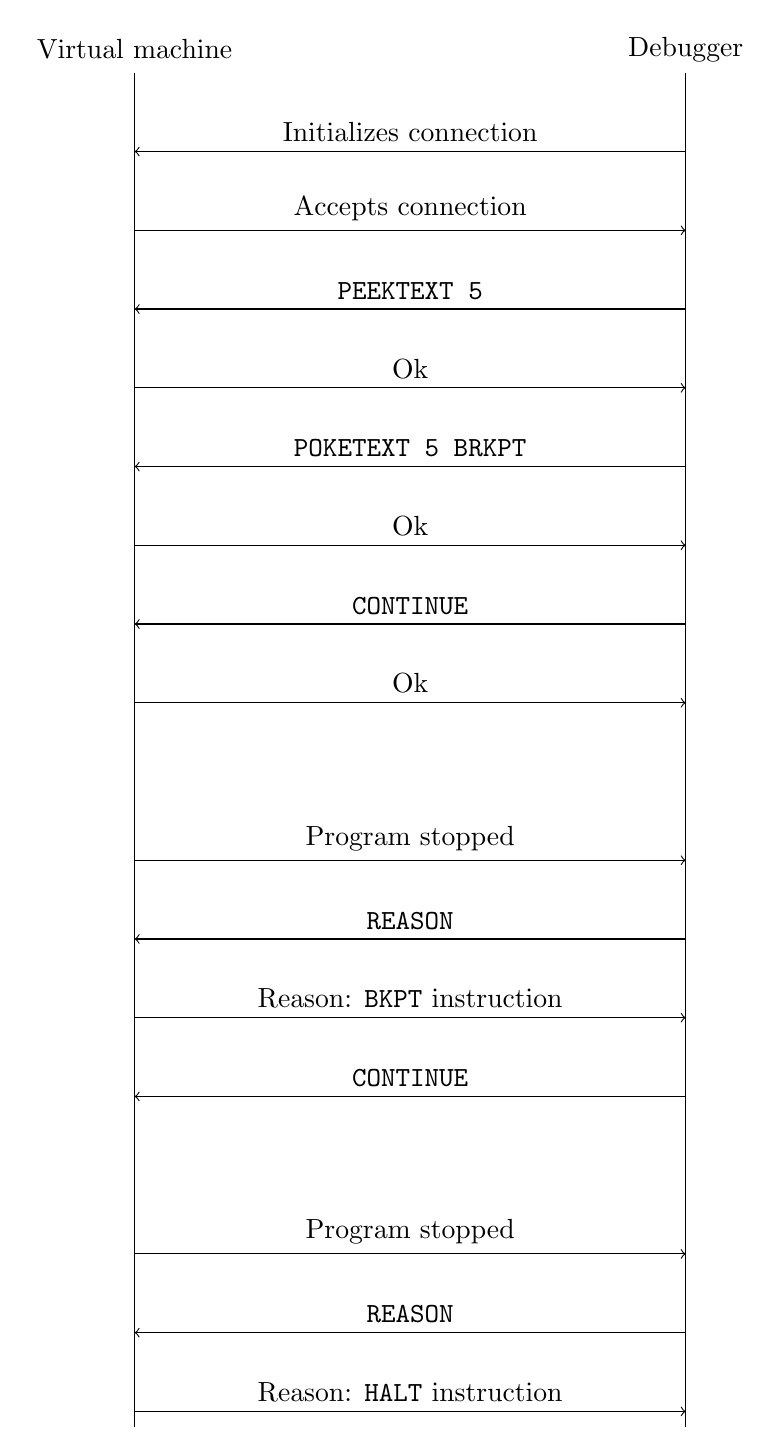
\begin{tikzpicture}
        \draw (0,0) -- (0,-17.2) (7,0) -- (7,-17.2);
        \node at (7,.3) {Debugger};
        \node at (0,.3) {Virtual machine};
        \draw[<-] (0,-1) -- node[midway,above] {Initializes connection} (7,-1);
        \draw[->] (0,-2) -- node[midway,above] {Accepts connection} (7,-2);
        \draw[<-] (0,-3) -- node[midway,above] {\texttt{PEEKTEXT 5}} (7,-3);
        \draw[->] (0,-4) -- node[midway,above] {Ok} (7,-4);
        \draw[<-] (0,-5) -- node[midway,above] {\texttt{POKETEXT 5 BRKPT}} (7,-5);
        \draw[->] (0,-6) -- node[midway,above] {Ok} (7,-6);
        \draw[<-] (0,-7) -- node[midway,above] {\texttt{CONTINUE}} (7,-7);
        \draw[->] (0,-8) -- node[midway,above] {Ok} (7,-8);
        \draw[->] (0,-10) -- node[midway,above] {Program stopped} (7,-10);
        \draw[<-] (0,-11) -- node[midway,above] {\texttt{REASON}} (7,-11);
        \draw[->] (0,-12) -- node[midway,above] {Reason: \texttt{BKPT} instruction} (7,-12);
        \draw[<-] (0,-13) -- node[midway,above] {\texttt{CONTINUE}} (7,-13);
        \draw[->] (0,-15) -- node[midway,above] {Program stopped} (7,-15);
        \draw[<-] (0,-16) -- node[midway,above] {\texttt{REASON}} (7,-16);
        \draw[->] (0,-17) -- node[midway,above] {Reason: \texttt{HALT} instruction} (7,-17);
    \end{tikzpicture}
    }
    \caption{A sequence diagram for the virtual machine and debugger communication.}
    \label{fig:dbg-vm-seq}
\end{figure}

